\section{System Background}

In this section, we introduce some fundamental concepts necessary to
understand the overall system design and the class of platforms
targeted by this work.

\subsection{Hybrid Multi-Core Platforms with Programmable Logic}
This work targets a class of embedded platforms that include
traditional full-speed embedded CPUs and programmable logic on the
same chip. This organization naturally defines two macro-domains,
namely the Processing Subsystem (PS) and the Programmable Logic
(PL). The PS encompasses a multi-core processor with a multi-level
cache hierarchy and a main memory (DRAM) controller. We use PS-PL
platforms to refer to this class of SoC for the reminder of this
work. A simplified block diagram for a reference PS-PL organization is
illustrated in Fig.~\ref{fig:PS-PL-diagram}. PS-PL platforms are
surging in popularity among manufacturers, researchers and industry
practitioners, with commercially available ARM-based products offered
by, most notably, Intel~\cite{stratix10} and
Xilinx~\cite{ultrascale+}. A pilot large-scale, high-performance PS-PL
system is the Enzian platform~\cite{enzian20} being rolled out by ETH
Zurich\footnote{Also see \url{http://enzian.systems/}}. Recently, a
RISC-V-based solution has been made available by Microsemi --- the
PolarFire SoC~\cite{icikle_kit}. \todo[inline][RM: we might want to
  move this part to the intro instead.]

\begin{figure}[ht!]
  \centering
  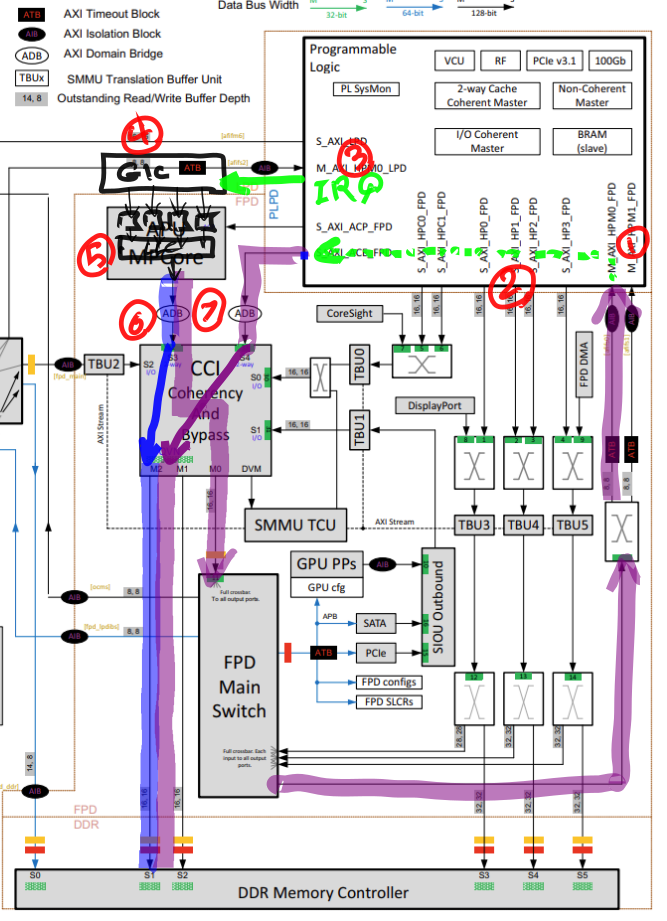
\includegraphics[scale=0.4]{images/ps-pl-interconnect.png}
  \caption{PS-PL interconnect block diagram}
  \label{fig:PS-PL-diagram}
\end{figure}

A key feature in PS-PL platforms is the presence of high-performance
communication channels between the two domains. These come in the form
of data exchange interfaces and interrupt lines. Data exchange
channels follow a master-slave paradigm. Specifically,
high-performance masters (HPM, \circledfig{fig:PS-PL-diagram}{1}) and high-performance
slaves (HPS, \circled{2})  send and receive transactions to and from
the PL, respectively. However, HPS's are not the only interface
mediums for PL-PS communications. The chip has (limited number of)
programmable interrupt lines \circled{3} present connected from the PL
to the generic interrupt controller (GIC), \circled{4}, inside the PS,
whereas the GIC is a primary resource for managing interrupts sent to
the processors. Like any other interrupt source in the system, a
unique ID number identifies each of the PL-PS interrupts lines. Hence,
by providing proper handlers associated with specific interrupt ID
lines and unmasking them, PL can request a desired service routine
from the PS. Nevertheless, as PS is buttressed by Arm Cortex-A53 Based
Application Processing Unit (APU), the interrupt controller supports
security extension to manage secure and non-secure interrupts grouped
by ARM TrustZone.


The underlying mechanism in this work is the ability to intercept
memory transactions originated from the processors inside the PS at
the PL. APU contains processing cores with private and shared caches
alongside a DRAM controller and I/O peripherals. A typical hierarchy
for modern embedded SoCs is to fabricate multi-level caches by arming
each processor with a private coherent L1 cache and having all
processors share a much larger L2 cache. The L2 cache is often also
the last-level cache (LLC). Upon a demand for data (or an
instruction), the cache is a premier location a processor scans for,
surmising for a copy of a required data tobe rapidly accessible, which
results in a cache hit. A miss results in the next cache level
look-up, and ultimately a miss in LLC provokes access to main memory.

While in caches with a write-through policy, the data gets
simultaneously written to the main memory as soon as it is updated in
the cache; caches with a write-back policy hold the most recent data
internally and write it back to the main memory only when it is
necessary, i.e., when the cache line is ready to replace. In this
sense, these transactions originate from the LLC toward the DRAM
\circled{5}. The cache controller is further in charge of determining
the replacement policy in the cache. Replacement policy effectively
resolves which cache line must be evicted when room for a new line is
needed. Conventional replacement policies for associative caches are
LRU, PLRU, FIFO, round-robin, and random.

While the straightforward route for main memory accesses is depicted
in Fig. \ref{fig:PS-PL-diagram} with blue highlight \circled{6}, the
PLIM technique introduces a secondary memory route for reaching the
DRAM, called Loop-Back. The application's memory traffic is
intercepted by dispatching them to leave the PS to enter the
PL. Intercepted transactions are then forwarded from the PL again
toward the memory controller inside the PS using an address
translation module. The primary mechanism of PS-PL and PL-PS
redirection of a transaction is called the Memory Loop-Back. Loop-Back
is done through address bit manipulation of the transaction such that
it falls in the range of the target HPM(HPS) for the PS-PL(PL-PS)
interception. In this way, the main memory content is accessed, but
through a programmable environment, highlighted in purple
\circled{7}. It is possible to act on the characteristics of the
traffic that now traverses the PL. For example, in the PL, it is
possible to direct the transaction to arbitrary modules before,
eventually, redirecting it back to PS and the memory controller,
ultimately.

This provides a unique capability of manipulating individual memory
transactions. Hence, by sitting between CPUs and main memory, PLIM is
exploited to perform memory scheduling. The idea is further leveraged
by designing a configurable memory scheduler in the middle, namely,
SchIM.

First and foremost, SchIM follows a selective and dynamic re-routing
policy settled at the run-time, meaning that provided a proper routing
configuration interface, SchIM can be bypassed if unacceptable
overhead for some applications is detected by going through the PL
following the Loop-Back routing strategy. Additionally, SchIM,
provides a safe production-ready environment on COTS platforms where
one can enfroce and test any proposed scheduling policy at the level
of the transaction altogether by the real hardware. Memory scheduling
traditionally done via hardware modifications at the controller level,
or solely via software. Providing SchIM, we are now able to transcend
this on intact COTS to conduct an analysis of feasibility, challenges
and performance.

In this paper we provide a several proof-cases where SchIM is
programmed to enforce a several elected scheduling policies of Fixed
Priority, TDMA, and Memguard.


\subsection{Jailhouse, the partitioning Hypervisor}
Jailhouse is a well-known open-source partitioning
hypervisor \footnote{The source code is available at
  \url{https://github.com/siemens/jailhouse.git}.} based on Linux,
with a prominent levity due to focusing on software-based partitioning
of only a handful of essential resources, i.e., on-chip resources like
CPUs, memory regions, I/O devices, and skipping any virtual
scheduling.

In Jailhouse's nomenclature, Virtual Machines (VMs) are referred to as
inmate cells where Jailhouse already supports colored mappings. An
inmate can be either a bare-metal application or any operating system
like Linux, each programmed to see a contiguous Intermediate Physical
Address (IPA) space. At the second stage, Jailhouse maps IPAs of
different cells to Physical Addresses (PAs) with a configurable color
specification. By doing so, Jailhouse supports the notion of temporal
partitioning wherein, by assigning a collection of non-overlapping
sets of processors to colored inmates, those cells cannot access a
(physical) address beyond their own address space resulting in
interference prevention.

Jailhouse gets enabled on top of a Linux, called root-cell, and uses a
configuration file associated with it to split off parts of the
system's resources and assign them to desired cells. Last but not
least, Jailhouse is especially useful since one can circumvent the
TrustZonce switches in any ARM-adapted OS (e.g., Linux), exploiting
the hypervisor calls.


\subsection{From Last-Level Cache to PL}
As illustrated in Fig. \ref{fig:PS-PL-diagram}, the considered system
features a Last-Level of Cache (or LLC) shared between the four cores
of the cluster. In the occurrence of a cache miss, the LLC controller
proceeds to access the targeted memory region by emitting an AXI
transaction. The exact size of the transaction (i.e., the amount of
burst) will vary depending on the size of the cache lines and the
width of the bus. The LLC acting as an intermediate and independent
module, it emits transactions that are not directly related to a
specific core. For instance, in the case of a cache line eviction, the
decision of which line to evict is done by the LLC controller
alone. In consequence, the emitted transactions do not carry the
information about the requesting cores as the LLC controller is the
only master. On ARM Cortex-A53 \ref{ARM-cortex-A53}, write
transactions (AWID) and read transactions (ARID) are respectivelly
tagged with IDs \verb|0b1xxxx| and \verb|0b1xxxnn| where \verb|xxxx|
is any number and \verb|nn| is the core ID.

\subsection{Advanced eXtensible Interface (AXI)}
\label{subsec:axi_transaction_scheme}
The Advanced eXtensible Interface (or AXI for short) is a widely
spread open specification bus protocol proposed by ARM \cite{ARM-AXI}
and exploited by Xilinx to interface both the PL side and the PS
side.\\ The AXI protocol is based on the master-slave
duality. Typically, the former is in charge of instantiating
transactions directed to any of the slaves composing the system.  On
the other hand, the latter, does not emit any transaction but receive
the requests emitted by a master and answer them.  The masters and the
slaves communicate between each other through five different channels
named AW, W, B, AR and R as illustrated in figure
\ref{fig:axi_transaction_scheme_figure}.  A write transaction will
start first by its address phase \circled{1}.  That is, the
transmission through the channel AW of meta-data regarding the
transaction such as the destination address, the transaction ID, the
amount of bursts and so on.  Upon the completion of this phase,
follows the data phase \circled{2} which, as its name suggests it,
consists in the transmission of the payload itself through the W
channel.  Thereafter, comes the response phase \circled{3} performed
on the B channel.  This phase, the only one being initiated by the
slave, is used to inform the master whether the transaction has been
completed successfully.  The transmission of a read transaction is
carried out in a similar way.  In fact, as for the writing, the
address phase \circled{1'} is transmitted through the equivalent
channel called AR and is directly followed by the data phase
\circled{2'}.  However, unlike the writing scheme, the data being
fetched, the data phase is instantiated by the slave.  The reading
response phase is performed simultaneously and is thus merge within
the R channel.\\ The protocol is said to be asynchronous as
transaction behaves similarly to packets each having a dedicated ID.
Hence, multiple outstanding transactions can be emitted successively
by a single master which can managed them in an out-of-order manner.

\begin{figure}
  \centering
  \begin{tikzpicture}[scale=0.5, every node/.style={scale=0.5}]
    % Module Master
    \draw ( 0.0, 0.0) -- ++( 2.0, 0.0) -- ++( 0.0, 5.25) -- ++( -2.0, 0.0);
    \node[rotate=90] at (0.25, 2.5) {\large MASTER};
    % Module Slave
    \draw (13.0, 0.0) -- ++(-2.0, 0.0) -- ++( 0.0, 5.25) -- ++( 2.0, 0.0);
    \node[rotate=270] at (12.75, 2.5) {\large SLAVE};
    % AW channel
    \node at ( 1.5, 4.50) {AW};
    \draw ( 2.0, 4.25) rectangle ++( 9.0, 0.5);
    \draw ( 5.0, 4.25) rectangle ++( 0.5, 0.5)  node[pos=.5] {A};
    \draw[-{Stealth}] ( 5.5, 4.5) -- ++( 0.5, 0.0);
    \node at ( 11.5, 4.50) {AW};
    \draw[red] ( 6.25, 4.50) circle [radius=0.2] node {1};
    % W channel
    \node at ( 1.5, 3.75) {W};
    \draw ( 2.0, 3.50) rectangle ++( 9.0, 0.5);
    \draw ( 3.0, 3.50) rectangle ++( 0.5, 0.5)  node[pos=.5] {D};
    \draw ( 3.5, 3.50) rectangle ++( 0.5, 0.5)  node[pos=.5] {...};
    \draw ( 4.0, 3.50) rectangle ++( 0.5, 0.5)  node[pos=.5] {D};
    \draw[-{Stealth}] ( 4.5, 3.75) -- ++( 0.5, 0.0);
    \node at ( 11.5, 3.75) {W};
    \draw[red] ( 5.25, 3.75) circle [radius=0.2] node {2};
    % B channel
    \node at ( 1.5, 3.00) {B};
    \draw ( 2.0, 2.75) rectangle ++( 9.0, 0.5);
    \draw ( 9.5, 2.75) rectangle ++( 0.5, 0.5)  node[pos=.5] {B};
    \draw[-{Stealth}] ( 9.5, 3.00) -- ++(-0.5, 0.0);
    \node at ( 11.5, 3.00) {B};
    \draw[red] ( 8.75, 3.00) circle [radius=0.2] node {3};
    % AR channel
    \node at ( 1.5, 1.50) {AR};
    \draw ( 2.0, 1.25) rectangle ++( 9.0, 0.5);
    \draw ( 5.0, 1.25) rectangle ++( 0.5, 0.5)  node[pos=.5] {A};
    \draw[-{Stealth}] ( 5.5, 1.5) -- ++( 0.5, 0.0);
    \node at ( 11.5, 1.50) {AR};
    \draw[red] ( 6.25, 1.50) circle [radius=0.2] node {1'};
    % R channel
    \node at ( 1.5, 0.75) {R};
    \draw ( 2.0, 0.50) rectangle ++( 9.0, 0.5);
    \draw ( 8.0, 0.50) rectangle ++( 0.5, 0.5)  node[pos=.5] {D};
    \draw ( 8.5, 0.50) rectangle ++( 0.5, 0.5)  node[pos=.5] {...};
    \draw ( 9.0, 0.50) rectangle ++( 0.5, 0.5)  node[pos=.5] {D};
    \draw ( 9.5, 0.50) rectangle ++( 0.5, 0.5)  node[pos=.5] {B};
    \draw[-{Stealth}] ( 8.0, 0.75) -- ++(-0.5, 0.0);
    \node at ( 11.5, 0.75) {R};
    \draw[red] ( 7.25, 0.75) circle [radius=0.2] node {2'};
\end{tikzpicture}

  \caption{Caption}
  \label{fig:axi_transaction_scheme_figure}
\end{figure}
